
\section{Background}\label{sec:background}

\subsection{Voice Acoustics}\label{sec:voice}

The generation of human voice follows a source-filter model~\cite{fant1960acoustic}. A speech signal can be seen as a source signal (the glottal source at the larynx, or noise generated at a constriction in the vocal tract), filtered with the resonances in the cavities of the vocal tract (tongue, teeth, lips, velum etc. modifying the sound spectrum over time). This theory has been verified using 3-D printed models of two configurations of a vocal tract to generate sounds to generate the vowels in the words ``had'' and ``heard''~\cite{wolfe2016experimentally}. 

%TODO choose one
%The fundamental frequency for speech ($f_0$) is typically 80 to 250 Hz.
A typical adult male will have a fundamental frequency  ($f_0$) of from 85 to 155 Hz, and that of a typical adult female from 165 to 255 Hz~\cite{baken1987clinical,titze1994principles}. The frequencies of the first, second and $i$-th resonances are labeled as  $R_1, R_2, \ldots R_i$, and those of the spectral peaks produced by these resonances are called formants, $F_1, F_2, \ldots F_i $~\cite{titze2015toward}. 
%
According to~\cite{ladefoged2014course}, English vowels are perceived largely according to the values of the formants $F_1$ and $F_2$. The range of $F_1$ is roughly from 270 to 860 Hz, and that of $F_2$ from 840 to 2790 Hz~\cite{peterson1952control}. As for English consonants, there are six categories: plosive/stop (e.g. /p/), fricative (e.g. /f/), affricate (e.g. /dZ/), nasal (e.g. /m/), lateral (e.g. /l/), and approximant (e.g. /r/). The frequencies of consonants vary a lot. The turbulence of /s/ and /z/ occurs above 3500Hz, and reaches as high as 10,000 Hz, whereas /w/ has $F_1$ from 250 to 450 Hz and $F_2 $ from 600 to 850 Hz~\cite{ladefoged2012vowels}. 

By Nyquist–Shannon sampling theorem, to properly sample a signal contains no frequency components higher than $f$ Hz, the sampling rate must be at least $2f$ Hz (Nyquist rate). In other words, a sampling rate of 400 Hz (motion sensors' rate as shown in Table~\ref{tab:sample}) can only handle signals whose component frequencies are below 200 Hz. Except for part of the fundamentals, all $F_1$ and $F_2$ frequencies can not be sensed. Therefore, it is impossible to perceive the signals with such a low sampling rate.
%
%The information of higher frequencies will be lost during the sampling stage.  
%Therefore, it is impossible to reconstruct the speech signals perfectly from motion sensor readings.   


%%TODO
However, borrowing theories from \textit{compressed sensing}, the {\systemName} system can partially reconstruct the signal and obtain critical information such as the numbers appeared in a conversation, genders or even identities of the speakers, etc., from motion sensor readings, as discussed in Section~\ref{sec:threat}.



%whose maximum frequency
%
%If a function 
%x(t) contains no frequencies higher than B hertz, it is completely determined by giving its ordinates at a series of points spaced 
%{1/(2B)} seconds apart.

%The sampling theorem indicates that a continuous signal can be properly sampled, only if it does not contain frequency components above one-half of the sampling rate. For instance, a sampling rate of 2,000 samples/second requires the analog signal to be composed of frequencies below 1000 cycles/second.

%Ladefoged, P. (2001). A Course in Phonetics (4TH EDITION). Boston, MA: Heinle and Heinle.
%
%In non-tonal languages such as English, vowels are perceived largely according to the values of the formants F1 and F2 in the sound (Peterson and Barney; 1952, Nearey, 1989; Carlson et al., 1970). F3 has a smaller role in vowel identification. F4 and F5 affect the timbre of the voice, but have little influence on which vowel is heard ((Sundberg, 1970). 
%
%A formant is a concentration of acoustic energy around a particular frequency in the speech wave. There are several formants, each at a different frequency, roughly one in each 1000Hz band. Each formant corresponds to a resonance in the vocal tract. We distinguish one vowel from another by the differences in these overtones. According to Lagefoged (2006), each vowel has three formants, i.e. three overtone pitches. The first formant (F1) is inversely related to vowel height. The second formant is related to the degree of backness of a vowel.
%Formants can be seen in a wideband spectrogram as dark bands.
%
%For singing, the range may be from about 60 Hz to over 1500 Hz, depending on the type of voice. 


%For example, at the larynx (sometimes called ‘voice box’), we produce a sound whose spectrum contains many different frequencies. Then, using tongue, teeth, lips, velum etc, (collectively called articulators) we modify the spectrum of that sound over time. In this simple introduction to the voice, we discuss the operations of first the ‘source’ of the sound, then of the ‘filter’ that modifies its spectrum, then of interactions between these.  
%
%The follows a Source-Filter model (Fant 1960)



\begin{figure}[!h]
	\centering
	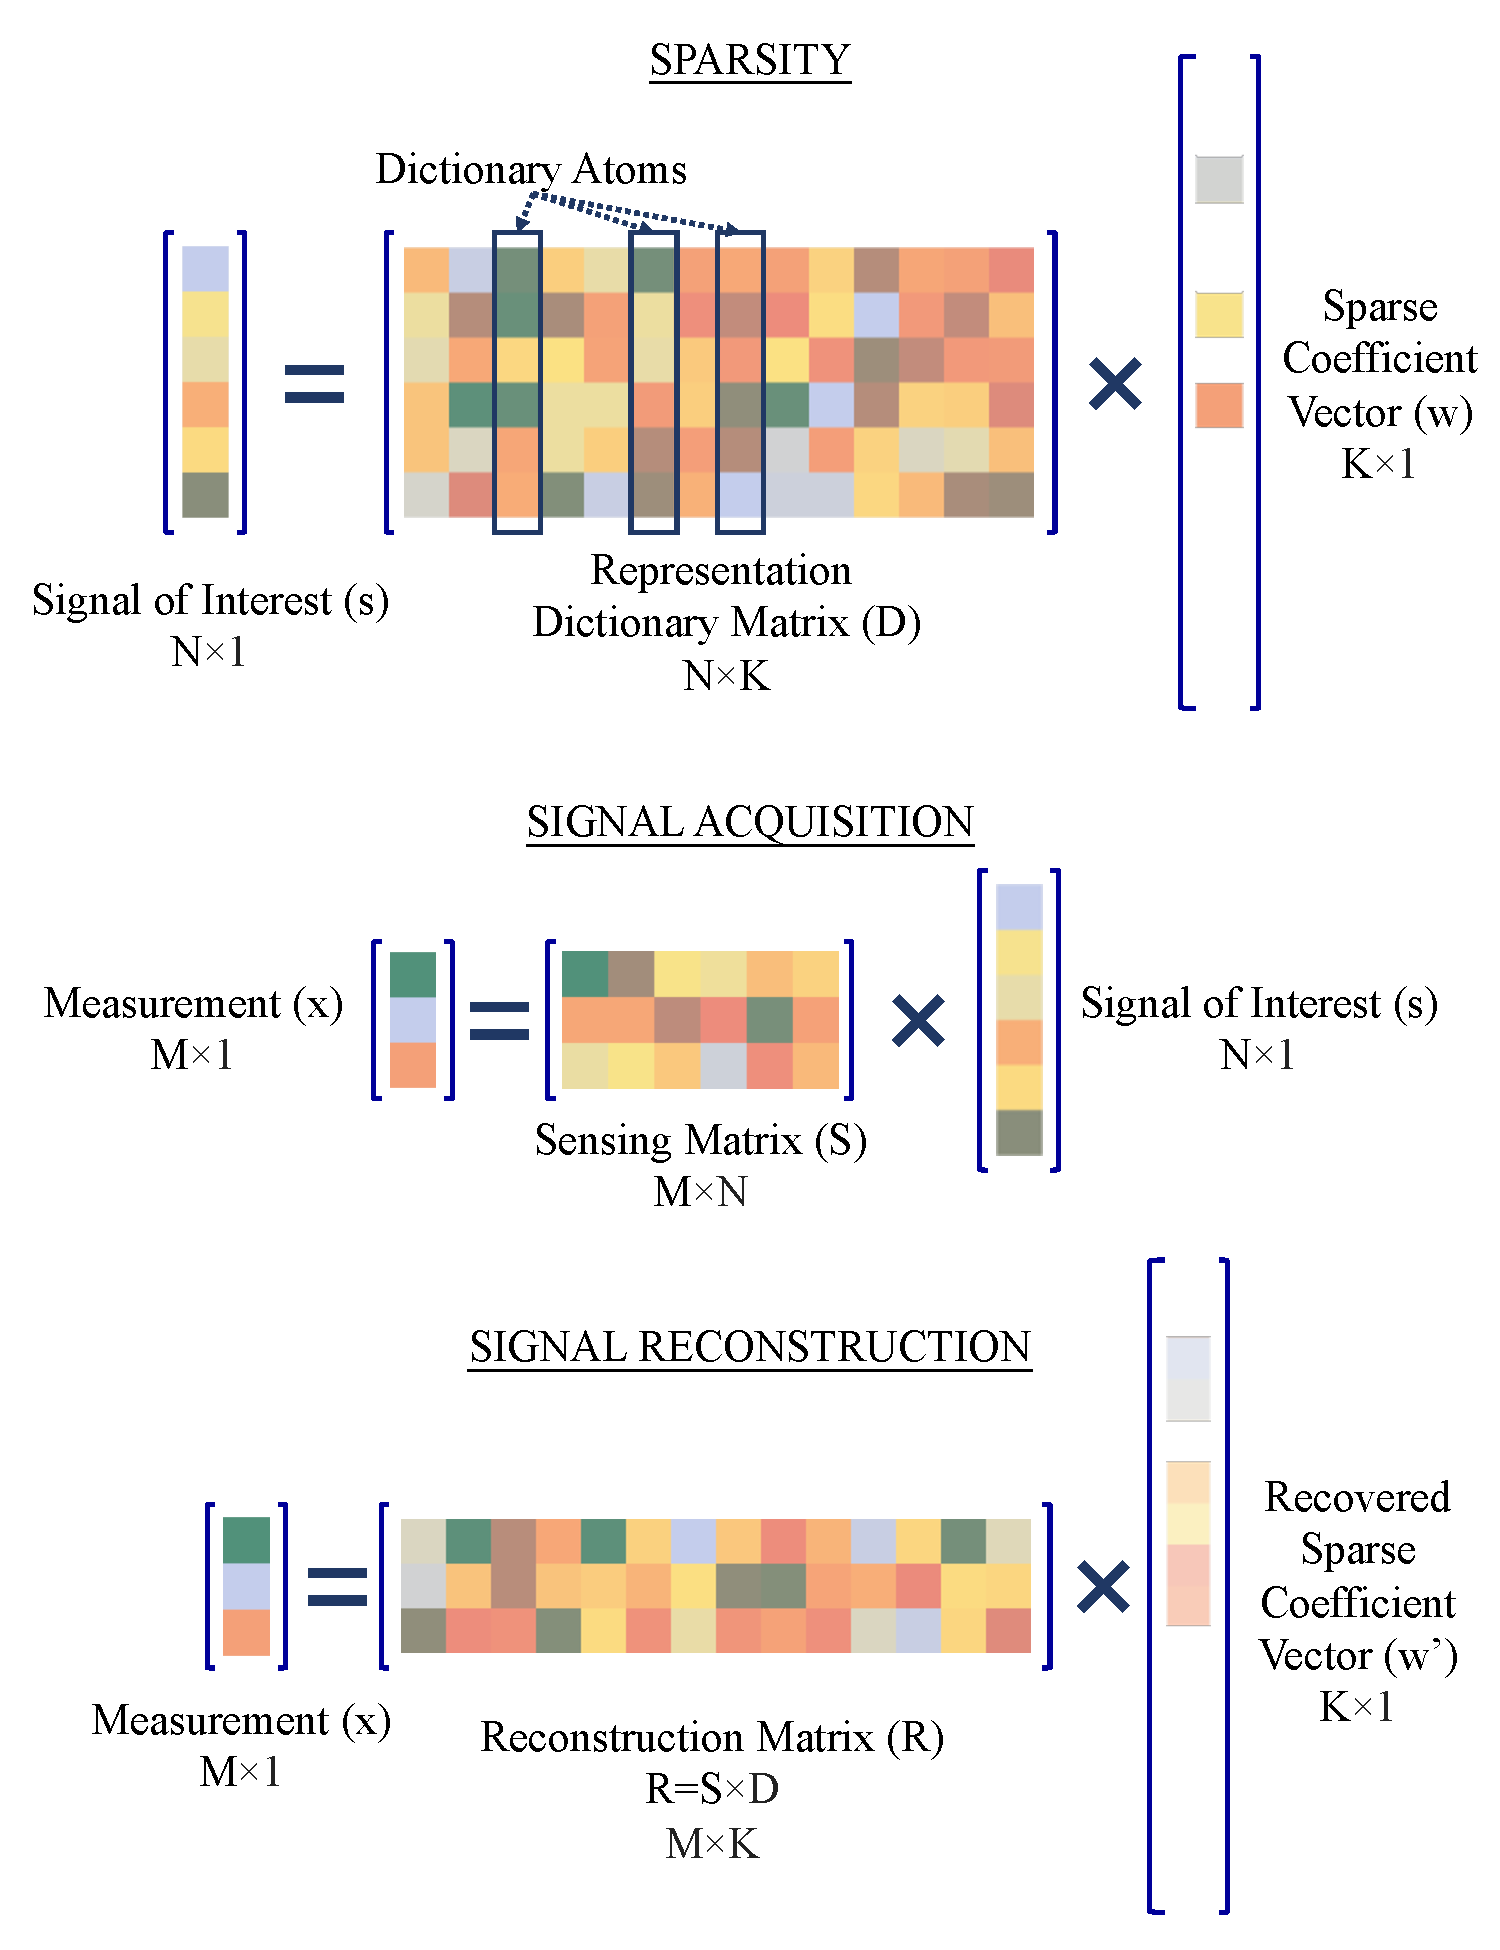
\includegraphics[width=.85\textwidth]{compressed}
	\caption{Mathematical Model of a Typical Compressed Sensing System. 
	}
	%		The signal of interest must be sparse (many zeros in the sparse coefficients vector $w$). In the signal acquisition stage, using a sensing matrix, the signal of interest is compressed to a measurement ($M \ll N$). In the signal reconstruction stage, a coefficient vector is recovered, which is an approximate of the original vector.}
	\label{fig:compressed}
\end{figure}

\subsection{Compressed Sensing}\label{sec:compressed}

%First introduced by Candes et al. in 2004~\cite{candes2004robust}, compressed sensing~\cite{donoho2006compressed} (also known as compressive sensing~\cite{siddamal2015survey}, compressive sampling~\cite{candes2006compressive}) is a novel signal acquisition and reconstruction technique. 
%
%Traditional methods requires the sampling rate to be at least 2 times the bandwidth of the signal (Nyquist rate). Compressed sensing, however, is capable of use far fewer samples while still perfectly (or nearly perfectly) recovering the signal. 


%Going against the established Nyquist–Shannon sampling theorem, compressed sensing 
%signal acquisition and reconstruction technique. 
Compressed sensing~\cite{donoho2006compressed} (also known as compressive sensing~\cite{siddamal2015survey}, compressive sampling~\cite{candes2006compressive}) is a novel sensing/sampling paradigm that acquires and reconstructs signals in a much more efficient way than the established Nyquist–Shannon sampling theorem. 

%Nyquist rate, it states that in order to obtain all relevant information in a signal, the sampling rate must be at least 2 times the bandwidth of the signal. 
%
%
% all relevant information in a signal The purpose of compressed sensing is to allow us to obtain fewer than the previously required amount of samples while still perfectly (or nearly perfectly) recovering the signal. 

First introduced by Candes et al. in 2004~\cite{candes2004robust}, compressed sensing takes advantage of prior knowledge about inherent characteristics (sparsity) of signals.
%constraints on the signal's frequencies. 
In this way, even with far fewer samples, the signal of interest can still be perfectly (or nearly perfectly) recovered. The constraint of Nyquist rate (sampling rate to be 2 times of signal bandwidth) is no longer a requirement. Therefore, we adopt this technique in the design of the  {\systemName} system.


As shown in Figure~\ref{fig:compressed}, the theory of compressed sensing has solid mathematical backgrounds. 
%
The signals of interest should have a low information rate, i.e., the signal is sparse in its original domain (e.g. time domain) or some transform domain (e.g. frequency domain)~\cite{candes2008introduction}. More precisely, when expressed in a proper representation dictionary $D$, a large number of coefficients in vector $w$ are zeros or small enough to be ignored. In fact, natural signals such as sound, image or seismic data have this sparsity property and can be stored in compressed form, in terms of their projection on suitable dictionary~\cite{qaisar2013compressive}. 

%Natural signals such as sound, image or seismic data can be stored in compressed form, in terms of their pro- jection on suitable basis. When basis is chosen properly, a large number of projection coefficients are zero or small enough to be ignored. If a signal has only s non-zero coefficients, it is said to be $s$-sparse.~\cite{qaisar2013compressive}

In the signal acquisition stage, compressed sensing aims to \textit{undersample} the signal of interest such that the dimension size $M$ of measurements $x$ is much smaller than the dimension size $N$ of the signal $s$. This goal is achieved by using a sensing matrix $S$ of size $M \times N$, where $M \ll N$.
%
The reconstruction of the original signal is essentially an optimization problem: 
%minimize $\Vert x - R w^\prime \Vert$ subject to number of non-zeros in $w^\prime$ smaller or equal to some threshold $\theta$. Here, the threshold $\theta$ defines how sparse the signal is. Mathematically, the objective of signal reconstruction in compressed sensing is to find
finding the optimal sparse coefficient vector
$w^\prime_{opt}$ such that 
\begin{equation}\label{eq:reconstruction}
w^\prime_{opt}
=
\argmin_{w^\prime}
\left( 
\gamma
\Vert w^\prime \Vert_p
+
\Vert x - R w^\prime \Vert_2
\right) 
,
\end{equation}
where $\gamma$ is the parameter to balance the evaluation weight of sparsity versus data error, $\Vert w^\prime \Vert_p$ is the $\ell_p$-norm of $w^\prime$, and $R$ is the reconstruction matrix which is equal to $S \times D$. As $\gamma$ increases the solution is getting more sparse. When $p=0$, this optimization problem has been proved to be NP-hard~\cite{natarajan1995sparse}. 


%0-norm (number of non-zeros) the 1-norm (sum of absolute values) or that the error (sum of squared errors) have reached a predefined limit. 





The overall performance of compressed sensing is determined by 3 aspects: how representative is the dictionary, how efficient is the sensing matrix, and how well-performed is optimization solver.
%
There are mainly two types of dictionaries, predefined dictionaries and learned dictionaries. Predefined dictionaries are built from basic functions like Fourier transform. Common dictionaries of this type include the discrete cosine transform basis, wavelet packages and Gabor bases~\cite{skretting2017sparse}. Learned dictionaries are learned from a training dataset of signals. Methods to build such type of dictionaries include K-SVD~\cite{aharon2006k}, MOD ILS-DLA~\cite{engan2007family}, ODL~\cite{mairal2009online}, RLS-DLA~\cite{skretting2010recursive}, and so on.
%Singular Value Decomposition K-SVD~\cite{aharon2006k}, Method of Optimized Directions (MOD) or the Iterative Least Squares Dictionary Learning Algorithm ILS-DLA~\cite{engan2007family}, the Online Dictionary Learning for Sparse Coding (ODL)~\cite{mairal2009online}, the Recursive Least Squares Dictionary Learning Algorithm (RLS-DLA)~\cite{skretting2010recursive}, and so on. 
%
As for the design of sensing matrix, it is important to check whether the matrix will allow the recovery of a sparse solution. The most famous one is the restricted isometry property ~\cite{candes2008restricted}, though it has been shown too strict~\cite{donoho2009observed}.
%
The signal reconstruction solvers span a wide series of techniques that include 
%matching pursuit/greedy, basis pursuit/linear programming, Matching Pursuit/Greedy, Basis Pursuit/Linear Programming, Bayesian, Iterative Thresholding, Proximal- . 
greedy pursuit, Bayesian framework, iterative thresholding, convex relaxation, nonconvex optimization, and brute force~\cite{tropp2010computational}. Some well-known solvers include
OMP~\cite{tropp2007signal}, GPSR~\cite{figueiredo2007gradient}, BCS~\cite{ji2008bayesian}, and so on. 
%orthogonal matching pursuit (OMP) ~\cite{tropp2007signal}, gradient projection sparse reconstruction (GPSR) ~\cite{bibid}, (BCS), and so on.
%LASSO, GPSR, BCS, ROMP, and so on.
%
More information can be found in survey papers like ~\cite{zhang2015survey,skretting2017sparse,rani2018systematic}.




In our attack design, the audio signals played from smartphone speakers are the signals of interest. When the sound is collected by motion sensors, it is essentially the signal acquisition stage that applies the sensing matrix to get the measurements. The motion data has a very low sampling rate, much lower than the Nyquist rate. However, using a carefully designed reconstruction matrix, the original signals of interest can be (partially) reconstructed from the recovered sparse coefficient vector and the representation dictionary ($s^\prime = D \times w^\prime$).
%
%More details will be illustrated in Section~\ref{sec:}.


%Techniques Used in Compressed sensing.
%
%Dictionary learning,
%MOD or ILS-DLA
%K-SVD
%ODL
%RLS-DLA
%
%ILS-DLA, the Iterative Least Squares Dictionary Learning Algorithm by Engan et al. ILS-DLA includes Method of Optimized Directions (MOD).
%K-SVD, the K-SVD method for dictionary learning by Aharon et al.
%RLS-DLA, the Recursive Least Squares Dictionary Learning Algorithm paper by Skretting and Engan.
%ODL, the Online Dictionary Learning for Sparse Coding paper by Mairal et al.
%SPAMS, the page for the SPArse Modeling Software by Mairal.



%Having said this, we are then interested in undersampled situations in which the number m of available measurements is much smaller than the dimension n of the signal f. 

%Based on this tenet, 
%
% When basis is chosen properly, a large number of projection coefficients are zero or small enough to be ignored. If  


%Sparsity expresses the idea that the “information rate” of a continuous time signal may be much smaller than suggested by its bandwidth, or that a discrete-time signal depends on a number of degrees of freedom which is comparably much smaller than its (finite) length. More precisely, compressive sampling exploits the fact that many natural signals are sparse or compressible in the sense that they have concise representations when expressed in the proper basis Ψ.

%a suitable basis or dictionary. D
%
% illustrates how 

%CS theory asserts that we can recover certain signals from fewer samples than required in Nyquist paradigm. This recov- ery is exact if signal being sensed has a low information rate (means it is sparse in original or some transform domain). Num- ber of samples needed for exact recovery depends on particular reconstruction algorithm being used. If signal is not sparse, then recovered signal is best reconstruction obtainable from s largest coefficients of signal. 
%
%When basis is chosen properly, a large number of projection coefficients are zero or small enough to be ignored. 
%Figure~\ref{fig:compressed} 
%
%
%use fewer samples than the common wisdom (Nyquist rate, 2 times of signal bandwidth) while still perfectly (or nearly perfectly) recovering the signal. The main idea is that with prior knowledge about constraints on the signal's frequencies, fewer samples are needed to reconstruct the signal.
%
% is built with solid mathematical background. 
%
%
%
%A signal can have sparse/compressible representation either in original domain or in some transform domains like Fourier transform, cosine transform, wavelet transform, etc. 
%
%proved that given knowledge about a signal's sparsity, the signal may be reconstructed with even fewer samples than the sampling theorem requires
%The theory of compresses sensing 
%
%
%This article surveys the theory of compressive sampling, also known as compressed sensing or CS, a novel sensing/sampling paradigm that goes against the common wisdom in data acquisition. CS theory asserts that one can recover certain signals and images from far fewer samples or measurements than traditional methods use. To make this possible, CS relies on two principles: sparsity, which pertains to the signals of interest, and incoherence, which pertains to the sensing modality. 
% 
% 
%
%Compressed sensing was introduced some ten years ago as an effective way of acquiring signals, which possess a sparse or nearly sparse representation in a suitable basis or dictionary. Due to its solid mathematical backgrounds, it quickly attracted the attention of mathematicians from several different areas, so that the most important aspects of the theory are nowadays very well understood. 
%
%
%The theory of compressive sensing was developed by Candes et al and Donoho in 2004. This method is different from traditional method as it sampled the signal below the Nyquist rate and it permits to exploit the sparse property at the signal acquisition stage of compression. In this method the signal is first transformed into a sparse domain and then the signal is reconstructed using numerical optimization technique using small number of linear measurements.
%
%%After the famous Shanon sampling theorem, introduction of compressive sensing (CS) is like a major breakthrough in signal processing community. CS was introduced by Donoho, Candès, Romberg, and Tao in 2004 [1]–[3].
%
%
%Compressive sensing (CS) is a novel sampling paradigm that samples signals in a much more efficient way than the estab- lished Nyquist sampling theorem. CS has recently gained a lot of attention due to its exploitation of signal sparsity. Sparsity, an in- herent characteristic of many natural signals, enables the signal to be stored in few samples and subsequently be recovered accu- rately, courtesy of CS. ~\cite{qaisar2013compressive}
%
%Compressed sensing (also known as compressive sensing~\cite{siddamal2015survey}, compressive sampling~\cite{candes2006compressive}, or sparse sampling) is a signal processing technique for efficiently acquiring and reconstructing a signal, by finding solutions to underdetermined linear systems. This is based on the principle that, through optimization, the sparsity of a signal can be exploited to recover it from far fewer samples than required by the Shannon-Nyquist sampling theorem. There are two conditions under which recovery is possible.[1] The first one is sparsity which requires the signal to be sparse in some domain. The second one is incoherence which is applied through the isometric property which is sufficient for sparse signals.
%
%A common goal of the engineering field of signal processing is to reconstruct a signal from a series of sampling measurements. In general, this task is impossible because there is no way to reconstruct a signal during the times that the signal is not measured. Nevertheless, with prior knowledge or assumptions about the signal, it turns out to be possible to perfectly reconstruct a signal from a series of measurements (acquiring this series of measurements is called sampling). Over time, engineers have improved their understanding of which assumptions are practical and how they can be generalized.
%
%An early breakthrough in signal processing was the Nyquist–Shannon sampling theorem. It states that if a real signal's highest frequency is less than half of the sampling rate (or less than the sampling rate, if the signal is complex), then the signal can be reconstructed perfectly by means of sinc interpolation. The main idea is that with prior knowledge about constraints on the signal's frequencies, fewer samples are needed to reconstruct the signal.
%
%Around 2004, Emmanuel Candès, Justin Romberg, Terence Tao, and David Donoho proved that given knowledge about a signal's sparsity, the signal may be reconstructed with even fewer samples than the sampling theorem requires.[4][5] This idea is the basis of compressed sensing.
\subsection{Smartphone Hardware}


\begin{figure}[!h]
	\centering
	\hspace{.25in}
	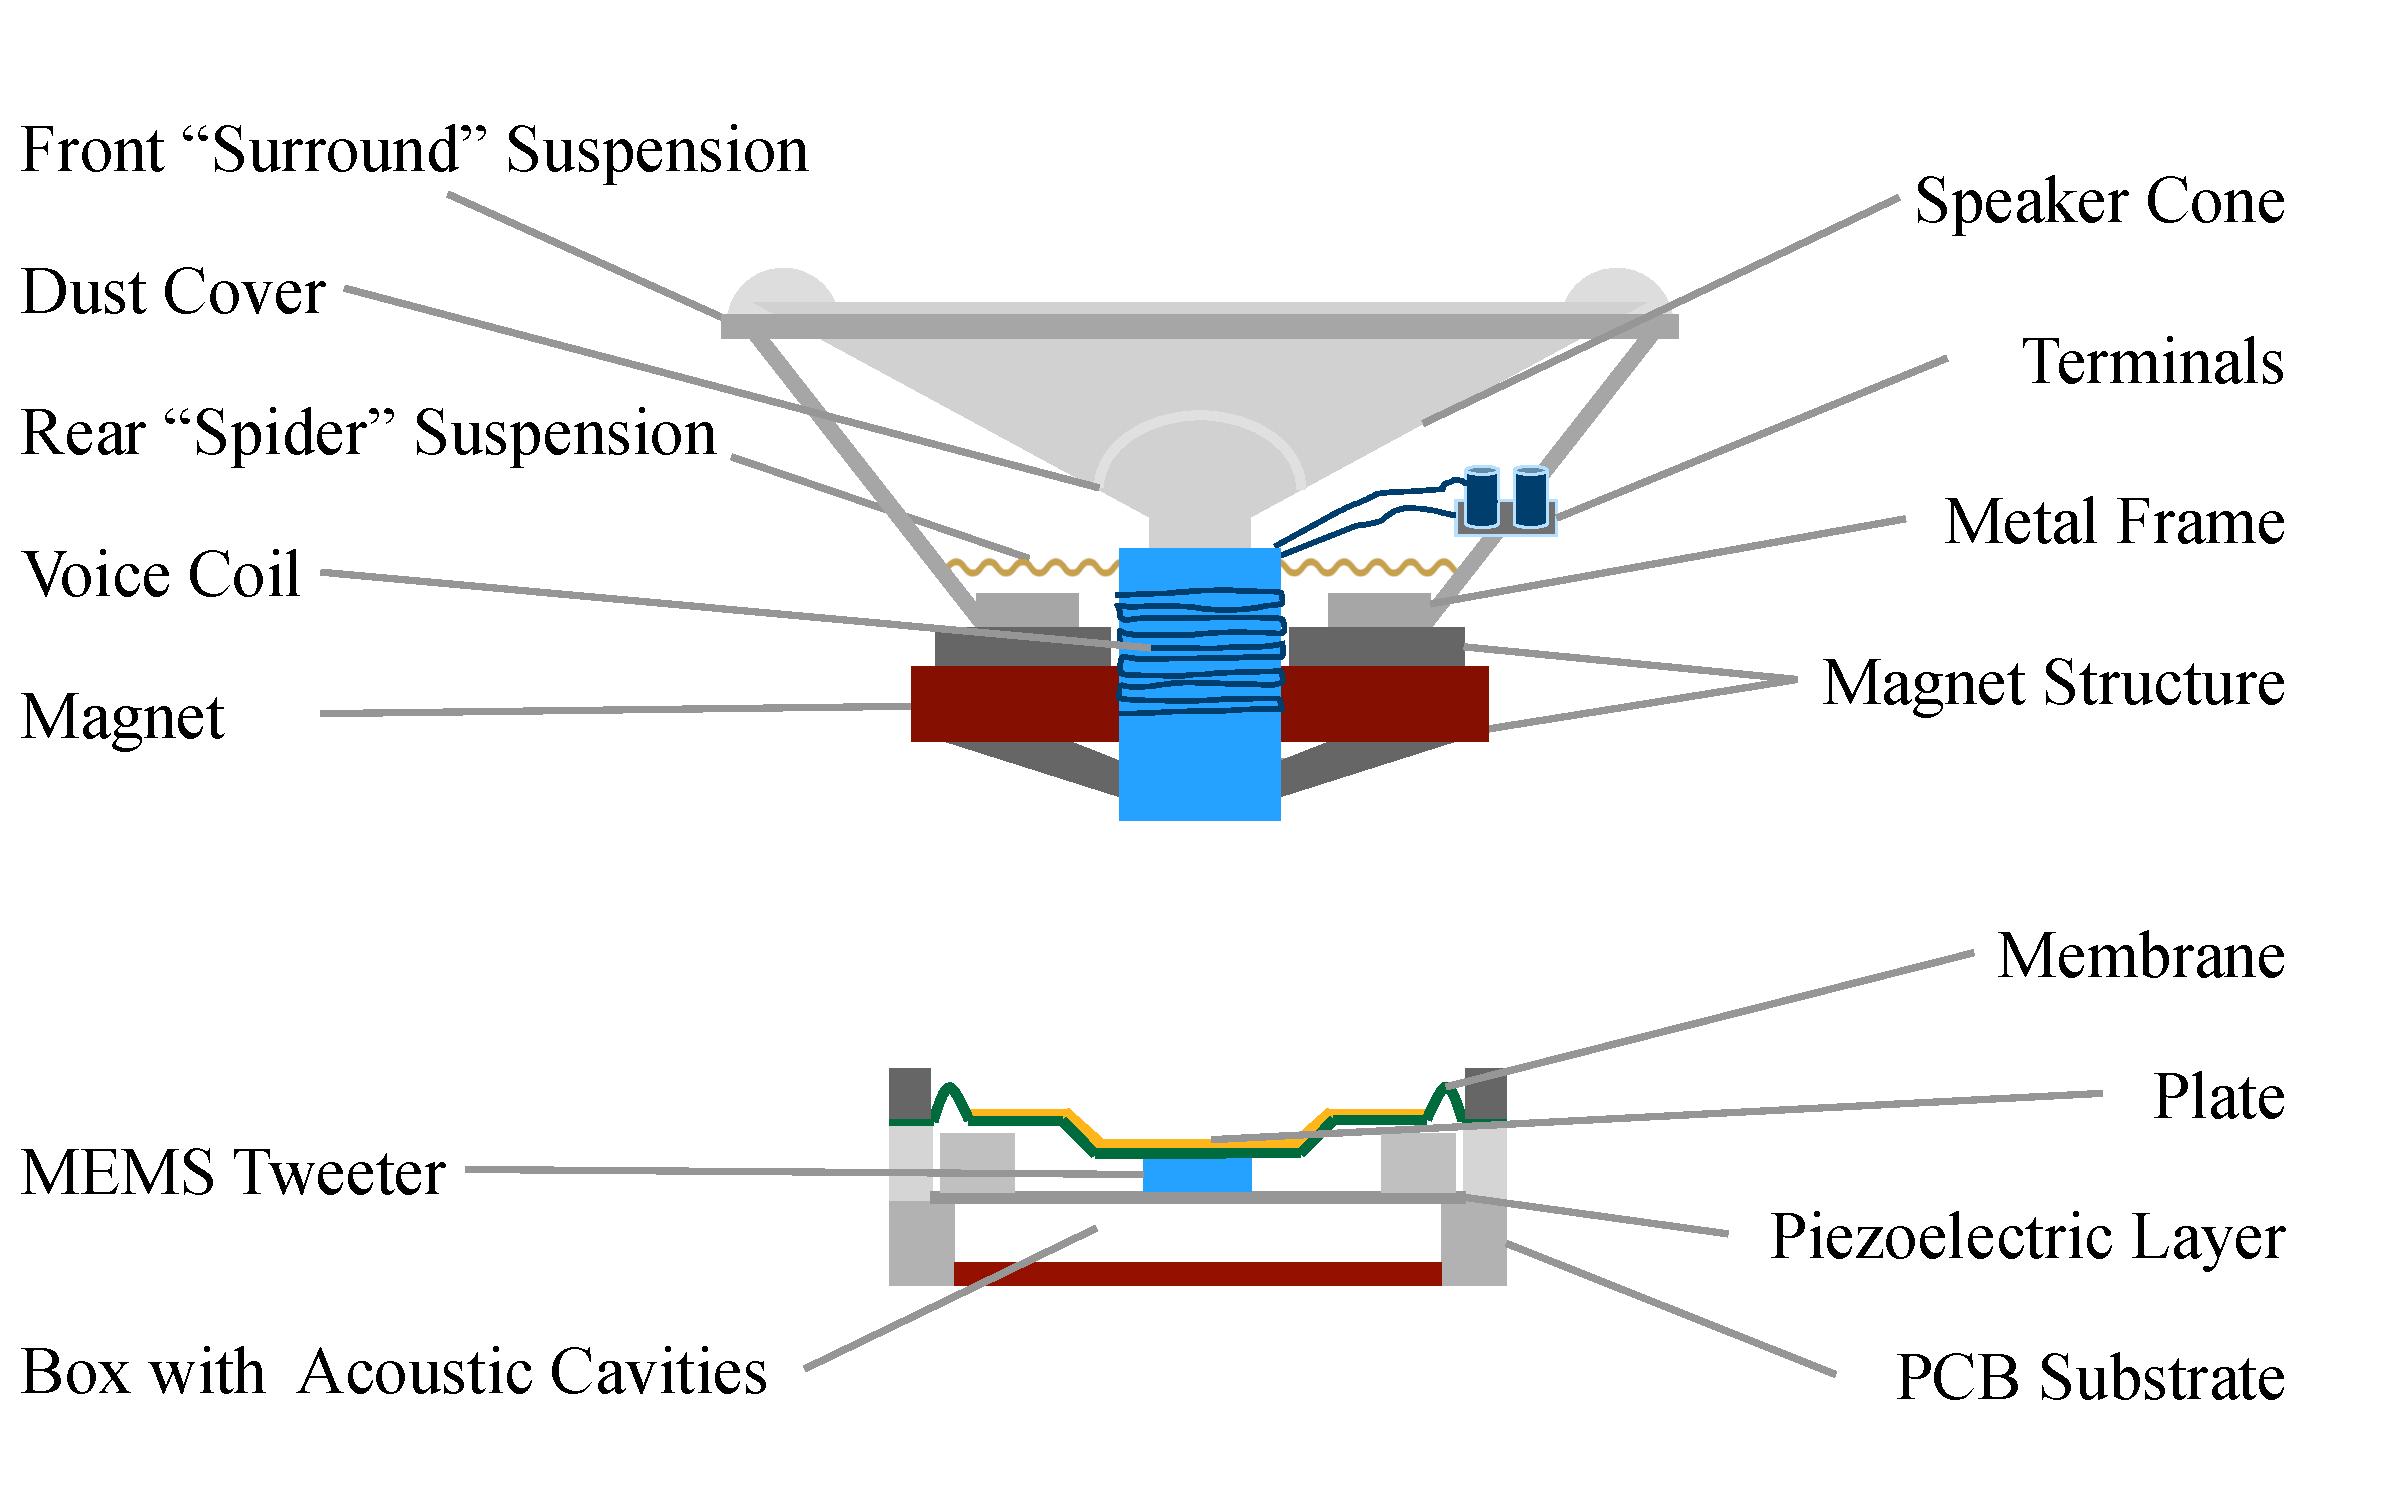
\includegraphics[width=.85\textwidth]{speaker}
	\caption{Structure of a Desktop Loudspeaker Versus an MEMS Speaker.}
	\label{fig:speaker}
\end{figure}

Figure~\ref{fig:speaker} shows the different structures of a typical desktop loudspeaker and a Micro Electro-Mechanical Systems (MEMS) speaker in smartphones. In desktop loudspeaker, sounds are created by alternating currents to the voice coil, while a smartphone speaker uses a small MEMS tweeter. As a result, the MEMS speaker consumes much less power than the desktop loudspeaker. But for the same reason, the sound pressure level (SPL) generated by MEMS speakers is much lower than that of desktop loudspeakers.


%%TODO

The Google Nexus 6P and Samsung Galaxy S8 used in this work can only generate sound with a maximum output of 78.4~dB
\footnote{\scriptsize \url{https://www.phonearena.com/phones/benchmarks}}. 
%\cite{onlinebenchmarks}.
The commercial off-the-shelf desktop loudspeaker, the \$22.99 Logitech Multimedia Speakers Z200 as an example, has max SPL greater than 88 dB. 
%
Note that a normal speech between two people typically has a range of 50 to 60 decibels and when they are shouting, the range goes to about 75 dB while 15\% of men can shout over 96 dB~\cite{online2005Voice}.
%
The higher the decibels, the easier for the motion sensors to catch the sound signals. With this respect, performing the {\attackName} attack is harder than Gyrophone~\cite{michalevsky2014gyrophone} or AccelWord~\cite{zhang2015accelword}.

As for the motion sensors, Google Nexus 6P uses Bosch BMI160, whose sampling rate can be 1600 Hz. However, the Android operating system only supports up to 400 Hz in order to save power.





% speakers and motion sensors
%Speakers on smartphones
%MEMES Speaker 
%MEMES IMU
%IMU sensor on smartphones
%
%Nexus4phonewhichaccordingtoateardownanal- ysis [13] is equipped with an InvenSense MPU- 6050 [12] gyroscope and accelerometer chip.
%2. Nexus 7 tablet which according to a teardown anal- ysis [14] is equipped with an InverSense MPU-6050 gyroscope and accelerometer.
%3. Samsung Galaxy S III phone which according to a teardown analysis [6] is equipped with an STMi- croelectronics LSM330DLC [10] gyroscope and ac- celerometer chip.

%In fact, these sensor-based threats highlight the flaws of existing sensor management systems used by smart devices. Specifically, Android sensor management sys- tem relies on permission-based access control, which considers only a few sensors (i.e., microphone, camera, and GPS)1. Android asks for access permission (i.e., with a list of permissions) only while an App is being installed for the first time. Once this permission is granted, the user has no control over how the listed sensors and other sensors (not listed) will be used by the specific App. Moreover, using some sensors is not considered as a vi- olation of security and privacy in Android. For instance, any App is permitted to access to motion sensors by just accessing the sensor API. Access to motion sensors is not controlled in Android.
%1IOS, Windows, and Blackberry also have permission-based sensor management systems. In this work, we focus on Android.


%loudness and sample rates
%
%%TODO
%Add a figure show how desktop speakers are much more powerful than MEMES
%dB compare  from
% \url{https://www.phonearena.com/reviews/Google-Nexus-6P-Review_id4110/page/3}
%
%speech recognition systems
%
%Nexus 6p Sampling Rate



